% Slide 02 — the list is stale and the visit is now.
%
% The slide used to be a visit timeline and a lot of white space. The visit
% strip alone never showed the thing that makes the list stale: the weeks
% behind it. So the top band is now that gap, carrying the four kinds of change
% that actually accumulate — a finished course, an over-the-counter purchase,
% a dose changed by someone else's doctor, a vaccination — and all of it funnels
% into the one dark box at the end of the visit.
%
% On the ~20 minutes: a site estimate, and a conservative one. Published
% medication-reconciliation times run far longer (a median of 50 minutes per
% patient; 46 at internal-medicine admission). It is labelled as an estimate
% because it is the only number in the deck without a citation.
%
% The load-bearing claim is the last line, and that one is corroborated:
% conmed data is entered at the site visit, which makes the record a test of
% what the participant can recall since the last one.
\documentclass[border=0pt]{standalone}
% Figure preamble: the shared base plus a transparent page background, so a
% figure composites onto the slide ground instead of carrying a white box.
% Shared preamble for every Reconmed figure and slide.
\usepackage{xcolor}
\usepackage{graphicx}
\usepackage{tikz}
\usetikzlibrary{positioning,calc,fit,backgrounds,shapes.misc,arrows.meta,decorations.pathreplacing}

% Reconmed — presentation palette.
%
% A green medical theme, derived from the product's tokens (frontend/src/styles/
% tokens.css) but with the brand moved to a deep clinical green.
%
% The product's colour rule survives the rebrand unchanged: warm hues (alarm,
% caution) are reserved for prohibited findings and low confidence — never for
% change types. Change types stay cool and are kept off the brand green so the
% brand and the "add" state do not blur together.
\definecolor{ground}{HTML}{EFF4F0}
\definecolor{surf}{HTML}{FFFFFF}
\definecolor{surfii}{HTML}{F6FAF7}
\definecolor{surfiii}{HTML}{E5EDE7}

\definecolor{line}{HTML}{DBE5DD}
\definecolor{lineii}{HTML}{C1D1C4}
\definecolor{lineiii}{HTML}{92A796}

\definecolor{ink}{HTML}{10231A}
\definecolor{inkii}{HTML}{3B4F43}
\definecolor{inkiii}{HTML}{66796D}
\definecolor{inkiv}{HTML}{92A796}

% the brand green
\definecolor{brand}{HTML}{14532D}
\definecolor{brandii}{HTML}{1B6B3A}
\definecolor{brandwash}{HTML}{E8F2EA}

% the participant side of the call — cool and neutral, so the agent's green
% is the only brand colour on the slide
\definecolor{patient}{HTML}{4E6570}

% change types — cool, deliberately unalarming
\definecolor{add}{HTML}{15803D}
\definecolor{stop}{HTML}{6A4C93}
\definecolor{modify}{HTML}{1F5FA8}
\definecolor{same}{HTML}{6B7C70}

% the one loud thing
\definecolor{alarm}{HTML}{C2190B}
\definecolor{alarmink}{HTML}{A3170C}
\definecolor{alarmdim}{HTML}{F1B9B2}
\definecolor{alarmwash}{HTML}{FDF3F1}

% low confidence — dim gold, never red
\definecolor{caution}{HTML}{8A6206}

\definecolor{accept}{HTML}{15803D}
% Rejected is a decision, not an alarm: kept neutral so red stays reserved for
% prohibited findings.
\definecolor{reject}{HTML}{5F6B72}

% Type for the deck.
%
% Two families: Montserrat for headings, big numbers and the wordmark — a
% geometric sans that reads as a health brand — over Open Sans for everything
% else. Keeping the body on Open Sans matters: the dense technical slides were
% measured against it, so the small type does not reflow under the rebrand.
\usepackage{fontspec}
\defaultfontfeatures{Ligatures=TeX}
\setsansfont{Open Sans}
\newfontfamily\displayfont{Montserrat}
\renewcommand{\familydefault}{\sfdefault}

% Shared TikZ styles. Every figure draws in millimetres (x=1mm,y=1mm) on a
% 160x90 canvas, so these sizes are literal.
%
% No blank lines may appear inside the \tikzset below: a blank line is \par,
% and the key parser will not tolerate it.
\tikzset{
  panel/.style     = {draw=line, fill=surf,   line width=0.4pt, rounded corners=2pt},
  panelgray/.style = {draw=line, fill=surfii, line width=0.4pt, rounded corners=2pt},
  screen/.style    = {draw=line, fill=surf,   line width=0.5pt, rounded corners=2.5pt},
  hair/.style      = {draw=line,   line width=0.4pt},
  hairii/.style    = {draw=lineii, line width=0.5pt},
  dimbar/.style    = {fill=line,   rounded corners=0.6pt},
  dimbarsm/.style  = {fill=lineii, rounded corners=0.5pt},
  lab/.style       = {font=\fontsize{7}{8.5}\selectfont\sffamily\color{inkiii}, inner sep=0pt, outer sep=0pt},
  val/.style       = {font=\fontsize{9}{11}\selectfont\sffamily\color{ink},    inner sep=0pt, outer sep=0pt},
  valb/.style      = {font=\fontsize{9}{11}\selectfont\sffamily\bfseries\color{ink}, inner sep=0pt, outer sep=0pt},
  code/.style      = {font=\fontsize{7}{8.5}\selectfont\ttfamily\color{inkiii}, inner sep=0pt, outer sep=0pt},
  tag/.style       = {font=\fontsize{5.6}{6.5}\selectfont\sffamily\bfseries, inner xsep=1.3mm, inner ysep=0.7mm, rounded corners=1.4pt},
  pill/.style      = {font=\fontsize{6.4}{7.5}\selectfont\sffamily\bfseries, inner xsep=1.5mm, inner ysep=0.85mm, rounded corners=1.5pt},
  headline/.style  = {font=\fontsize{12}{14}\selectfont\sffamily\bfseries\color{ink}, anchor=west, inner sep=0pt, outer sep=0pt},
  subline/.style   = {font=\fontsize{7.5}{9}\selectfont\sffamily\color{inkii}, anchor=west, inner sep=0pt, outer sep=0pt},
  cardlab/.style   = {font=\fontsize{6.4}{7.5}\selectfont\sffamily\color{inkiii}, anchor=west, inner sep=0pt, outer sep=0pt},
  num/.style       = {font=\fontsize{22}{23}\selectfont\sffamily\bfseries\color{ink}, anchor=west, inner sep=0pt, outer sep=0pt},
  flow/.style      = {-{Stealth[length=1.5mm,width=1.2mm]}, draw=lineii, line width=0.7pt},
}

% The conmed mark.
%
% Concept: two records — the log on file, and what the participant said —
% converging into a single reconciled line. Drawn once as a standalone asset
% (shared/marks/conmed.tex) so it scales cleanly: PDF inclusion scales the
% strokes, which TikZ scope scaling would not.
\newcommand{\conmedmark}[1][16mm]{
\includegraphics[height=#1]{shared/marks/conmed.pdf}}


\AtBeginDocument{\ifdefined\nopagecolor\nopagecolor\fi}

\begin{document}
\hyphenpenalty=10000\exhyphenpenalty=10000
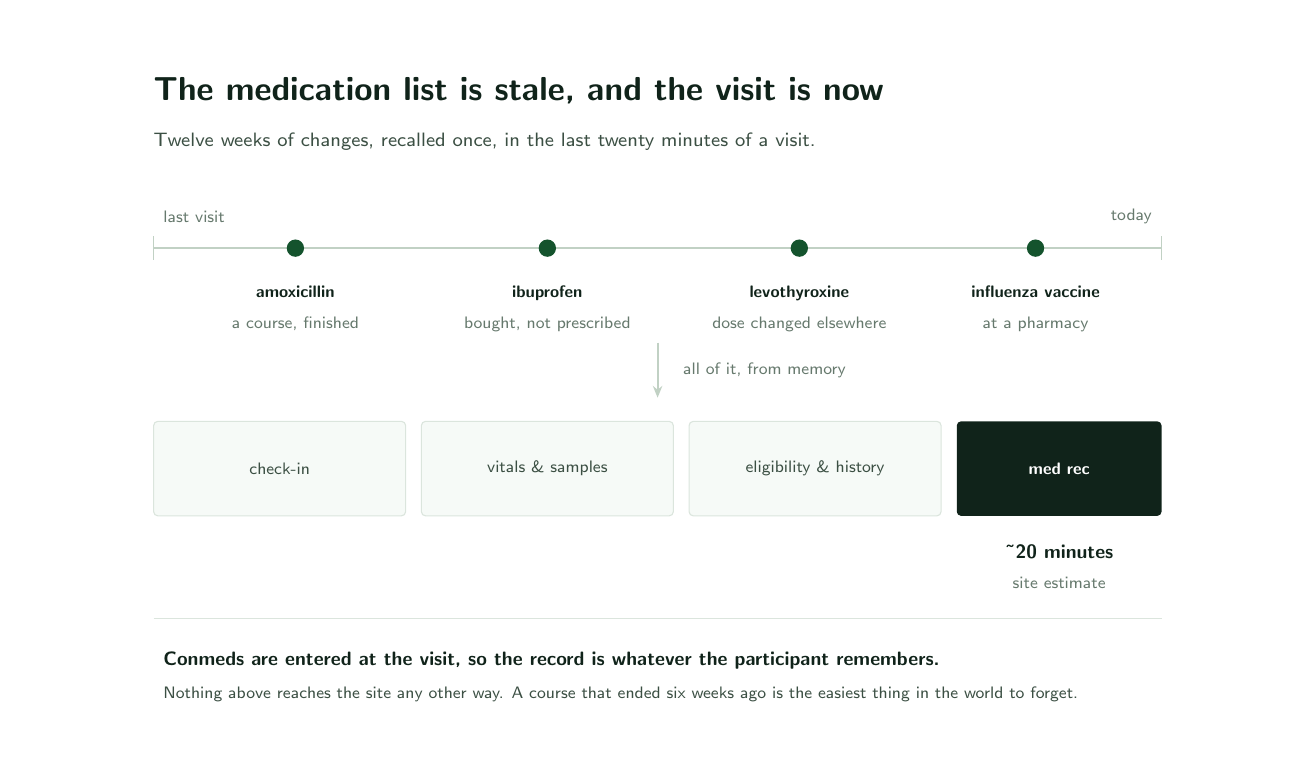
\begin{tikzpicture}[x=1mm,y=1mm]
\path[use as bounding box] (0,0) rectangle (160,90);

\node[headline] at (16,82) {The medication list is stale, and the visit is now};
\node[subline]  at (16,75.5) {Twelve weeks of changes, recalled once, in the last twenty minutes of a visit.};

% ---- the gap between visits --------------------------------------------
\node[anchor=west, font=\fontsize{6}{7.2}\selectfont\sffamily\color{inkiii}] at (16,66) {last visit};
\node[anchor=east, font=\fontsize{6}{7.2}\selectfont\sffamily\color{inkiii}] at (144,66) {today};
\draw[hairii] (16,62) -- (144,62);
\draw[hairii] (16,60.5) -- (16,63.5);
\draw[hairii] (144,60.5) -- (144,63.5);

\foreach \x/\what/\why in {%
  34/{amoxicillin}/{a course, finished},
  66/{ibuprofen}/{bought, not prescribed},
  98/{levothyroxine}/{dose changed elsewhere},
  128/{influenza vaccine}/{at a pharmacy}} {
  \fill[brand] (\x,62) circle (1.1);
  \node[anchor=north, font=\fontsize{6.4}{7.7}\selectfont\sffamily\bfseries\color{ink}] at (\x,58.5) {\what};
  \node[anchor=north, font=\fontsize{5.8}{7}\selectfont\sffamily\color{inkiii}] at (\x,54.5) {\why};
}

% ---- it all funnels into one box ---------------------------------------
\draw[flow] (80,50) -- (80,43);
\node[anchor=west, font=\fontsize{6}{7.2}\selectfont\sffamily\color{inkiii}] at (82,46.5) {all of it, from memory};

% ---- the visit ----------------------------------------------------------
\foreach \x/\w/\lab in {16/32/{check-in}, 50/32/{vitals \& samples}, 84/32/{eligibility \& history}} {
  \fill[surfii, draw=line, line width=0.4pt, rounded corners=1.5pt] (\x,28) rectangle (\x+\w,40);
  \node[font=\fontsize{6.2}{7.5}\selectfont\sffamily\color{inkii}] at (\x+\w/2,34) {\lab};
}
\fill[ink, rounded corners=1.5pt] (118,28) rectangle (144,40);
\node[font=\fontsize{6.2}{7.5}\selectfont\sffamily\bfseries\color{white}] at (131,34) {med rec};

\node[anchor=north, font=\fontsize{7.2}{8.6}\selectfont\sffamily\bfseries\color{ink}] at (131,25.5) {\textasciitilde20 minutes};
\node[anchor=north, font=\fontsize{5.8}{7}\selectfont\sffamily\color{inkiii}] at (131,21.5) {site estimate};

% ---- the claim ----------------------------------------------------------
\draw[line, line width=0.5pt] (16,15) -- (144,15);
\node[anchor=north west, font=\fontsize{7.4}{9}\selectfont\sffamily\bfseries\color{ink}] at (16,12)
  {Conmeds are entered at the visit, so the record is whatever the participant remembers.};
\node[anchor=north west, font=\fontsize{6.2}{7.5}\selectfont\sffamily\color{inkii}] at (16,7.5)
  {Nothing above reaches the site any other way. A course that ended six weeks ago is the easiest thing in the world to forget.};

\end{tikzpicture}
\end{document}
